% Evidence-bounded IEEE draft. This is not a submission-ready manuscript.
% Do not rename this file to main.tex until the gates in main_tex_preflight.md pass.
\documentclass[journal]{IEEEtran}

\usepackage{cite}
\usepackage{graphicx}
\usepackage{booktabs}
\usepackage{array}
\usepackage{amsmath}
\usepackage{amssymb}
\usepackage{url}
\usepackage[hidelinks]{hyperref}

\graphicspath{{../figures/scale_analysis/}{../figures/method/}{figures/}}

\begin{document}

\title{High-Resolution Prediction for Lightweight UAV Small-Object Detection: Evidence, Validity Boundaries, and Cross-Scale Adaptation}

\author{First~Author,
        Second~Author,
        and~Third~Author}

\markboth{IEEE Transactions,~Vol.~XX, No.~XX, 2026}%
{High-Resolution Prediction for Lightweight UAV Small-Object Detection}

\maketitle

\begin{abstract}
Lightweight detectors are attractive for unmanned aerial vehicle (UAV) traffic perception, but dense small road users are easily weakened by repeated downsampling. This paper studies high-resolution prediction for YOLO11n-family UAV small-object detection under a traceable VisDrone2019-DET/UAVDT protocol. We first separate input-resolution and prediction-scale effects. On VisDrone, increasing YOLO11n input from 640 to 960 improves mAP50--95 from 0.182 to 0.251. With matched 960 input, a static P2 branch raises mAP50--95 from 0.251 to 0.256 and small-object recall from 0.420 to 0.450, but increases computation from 6.5 to 10.7 GFLOPs and does not dominate all scale bins. Cross-dataset evaluation further shows a validity boundary: YOLO11n-P2-960 obtains 0.539 mAP50--95 on UAVDT, below YOLO11n-960 (0.591), YOLOv8n-960 (0.595), and YOLO11s-960 (0.608). A first adaptive gate, ScaleAwareP2Gate, remains mixed/negative evidence. Motivated by this failure, CrossScaleP2P3ConsistencyGate (CSGate) conditions P2 detail on adjacent P3 semantics. CSGate reaches 0.272 mAP50--95 and 0.456 small-object recall on VisDrone, and 0.567 mAP50--95 on UAVDT, repairing 54.8\% of the static-P2 degradation. The claim is therefore a bounded cross-scale adaptation method, not a state-of-the-art or universal-transfer assertion.
\end{abstract}

\begin{IEEEkeywords}
UAV object detection, small object detection, lightweight YOLO, high-resolution prediction, scale-wise analysis, VisDrone.
\end{IEEEkeywords}

\section{Introduction}

Unmanned aerial vehicles provide flexible viewpoints for traffic monitoring, emergency response, and urban scene understanding. In these scenes, pedestrians, vehicles, and non-motorized traffic participants often appear as small targets under oblique or top-down viewpoints. Dense layouts, occlusion, scale variation, and background clutter make the detection problem different from ordinary ground-view object detection. For traffic-oriented UAV perception, missing small road users can be more consequential than a small change in an aggregate metric, while practical deployment still requires a compact and efficient detector.

Lightweight YOLO models are attractive because they reduce parameters, storage, and inference cost. However, their compact feature hierarchy also creates a tension: repeated downsampling improves semantic abstraction but can weaken the spatial detail needed by tiny objects. Increasing input resolution and adding a shallow high-resolution prediction branch are intuitive remedies, but they are not free. They may increase computation, change the precision-recall balance, or improve small-object diagnostics at the cost of medium/large-object behavior. Therefore, the central question is not simply whether a P2 branch can be added to YOLO11n, but when high-resolution prediction helps a lightweight UAV detector and what price it pays.

This paper studies that question using YOLO11n as the nano-scale reference. Instead of treating P2, CoordAttention, TOFC, and training-augmentation variants as a collection of unrelated improvements, we organize them around three research questions:

\begin{itemize}
  \item \emph{Resolution effect:} how much of the improvement comes from increasing the effective image resolution for small targets?
  \item \emph{Prediction-scale effect:} after matching the input resolution, does a P2 high-resolution branch provide additional small-object benefit?
  \item \emph{Validity boundary:} do attention and feature-calibration variants provide consistent gains, or are their effects metric- and dataset-dependent?
\end{itemize}

The same logic also guides the adaptive-gate redesign. A static P2 branch is useful only if its shallow spatial detail remains compatible with the target data distribution. If the branch improves one dataset but degrades another, the method question becomes more specific: how should a lightweight detector retain P2 detail without allowing local shallow cues to dominate when the dataset favors different scale statistics? ScaleAwareP2Gate and CSGate are evaluated under this question rather than introduced as isolated architectural additions.

The completed VisDrone2019-DET evidence suggests that high-resolution input is the dominant gain source for YOLO11n, and that the P2 branch provides additional small-object diagnostic improvement under matched 960 input. The completed UAVDT comparison, however, shows that this P2 trend does not transfer under the current setting. Together, the results show clear boundaries: the VisDrone gain is modest in aggregate mAP, the P2 branch increases GFLOPs, CoordAttention and TOFC behave differently across metrics, and larger or alternative lightweight baselines remain stronger on UAVDT. These observations motivate a study framed around benefits, costs, and validity boundaries, not an overstated best-performance claim.

The contributions are:

\begin{itemize}
  \item A traceable experimental analysis of high-resolution prediction for lightweight YOLO-family detectors on VisDrone2019-DET, with UAVDT used as a cross-dataset validity-boundary test.
  \item A scale-wise diagnostic protocol that reports recall/precision and local scale-bin AP, clarifying how high-resolution prediction affects small, medium, and large objects beyond aggregate mAP.
  \item An accuracy-efficiency analysis that jointly reports mAP, parameters, GFLOPs, weight size, latency, and FPS, exposing the cost of P2 and calibration variants.
  \item A completed adaptive-gate study showing that ScaleAwareP2Gate is mixed/negative evidence, while CrossScaleP2P3ConsistencyGate passes the predeclared cross-dataset repair and small-object diagnostic routes without supporting an unbounded superiority claim.
\end{itemize}

\section{Related Work}

\subsection{UAV Object Detection Benchmarks}

UAV object detection benchmarks provide the basis for evaluating aerial traffic perception and small-object detection. VisDrone2019-DET contains diverse UAV-captured scenes and has been widely used for drone-view object detection evaluation \cite{du2019visdrone_det}. UAVDT emphasizes vehicle detection and tracking in UAV traffic scenes \cite{du2018uavdt}. Other aerial or UAV-related datasets, including AI-TOD, TinyPerson, AU-AIR, and HIT-UAV, further highlight tiny-object, low-altitude traffic, and modality-specific detection challenges \cite{wang2021aitod,xu2022aitodv2_nwd,yu2020tinyperson,bozcan2020auair,suo2023hituav}. These datasets expose small scale, occlusion, density, and viewpoint variation, which are central to lightweight detector design.

\subsection{Feature Pyramids and High-Resolution Prediction}

Feature pyramid designs improve multi-scale representation by combining semantic and spatial information across feature levels. FPN \cite{lin2017fpn}, PANet \cite{liu2018panet}, and EfficientDet \cite{tan2020efficientdet} are representative examples of multi-scale feature fusion. For UAV images, shallow high-resolution features are especially relevant because tiny objects may disappear or become ambiguous in deep low-resolution maps. Drone-view YOLO variants often strengthen high-resolution detection heads, multi-scale aggregation, or attention-based recalibration to address this problem \cite{zhu2021tph_yolov5,li2024sod_yolo,khalili2024sod_yolov8,qu2025sma_yolo,lu2025masf_yolo,xu2025srtsod_yolo}. This literature also increases the novelty requirement for the present work: a P2 branch or attention module alone should be positioned as a measured design choice unless additional evidence supports a stronger methodological claim.

\subsection{Lightweight YOLO Detectors and Attention}

YOLO-family detectors are widely used when real-time or near-real-time detection is required. Compact models reduce parameters and storage, but dense small-object scenes remain challenging. Attention modules can recalibrate feature responses with limited overhead. Coordinate Attention encodes positional information into lightweight attention maps \cite{hou2021coordinate_attention}, but its empirical contribution must be interpreted from measured results rather than assumed. For this reason, this study treats attention and feature-calibration modules as ablations unless both aggregate and scale-wise diagnostics support their role.

\subsection{Position of This Study}

The related methods in Table~\ref{tab:ieee_literature_context} show that recent UAV small-object detectors commonly strengthen high-resolution heads, multi-scale fusion, attention, or lightweight YOLO backbones. This creates two requirements for the present work. First, the manuscript should not claim novelty from the mere presence of an extra shallow prediction head or an attention block. Second, any adaptive high-resolution design must be justified by diagnostic evidence that separates input resolution, prediction scale, model capacity, and cross-dataset behavior. The contribution is therefore positioned as an evidence-bounded study and method refinement: static P2 is analyzed as a measured design choice, ScaleAwareP2Gate is retained as a negative/mixed adaptive-gate case, and CSGate is promoted only to the extent supported by the accepted repair and small-object diagnostic routes.

% Auto-generated by tools/export_ieee_tables.py.
% Values are copied from audited CSV files; do not edit numbers by hand.
\begin{table}[t]
\centering
\caption{Literature context for recent UAV small-object YOLO methods.}
\label{tab:ieee_literature_context}
\footnotesize
\begin{tabular}{llrp{0.28\linewidth}p{0.28\linewidth}}
\hline
Work & Key & Year & Focus & Use \\
\hline
TPH-YOLOv5 & zhu2021tph\_yolov5 & 2021 & YOLOv5 with extra detection heads and Transformer prediction head & High-resolution/head-design prior \\
SOD-YOLO & li2024sod\_yolo & 2024 & Improved YOLOv8 for UAV small objects & Recent UAV YOLOv8 prior \\
SOD-YOLOv8 & khalili2024sod\_yolov8 & 2024 & YOLOv8 for aerial imagery and traffic small objects & T-ITS-relevant traffic/aerial prior \\
SMA-YOLO & qu2025sma\_yolo & 2025 & YOLOv8 with parameter-free attention and multi-scale fusion & Recent multi-scale UAV YOLOv8 prior \\
MASF-YOLO & lu2025masf\_yolo & 2025 & YOLO11-based multi-scale aggregation and adaptive fusion & Close YOLO11 novelty-pressure prior; preprint \\
SRTSOD-YOLO & xu2025srtsod\_yolo & 2025 & YOLO11-based real-time UAV small-object detection & Strong recent YOLO11 prior \\
\hline
\end{tabular}
\vspace{1mm}\par\footnotesize This table is for related-work context only. It does not contain reproduced performance values or a direct ranking.
\end{table}


\section{Evidence-Bounded Cross-Scale High-Resolution Prediction}

\subsection{Problem Formulation}

Let \(x\) denote a UAV image and \(f_{\theta}(x;s,\mathcal{H})\) denote a lightweight detector with parameters \(\theta\), input size \(s\), and prediction-head set \(\mathcal{H}\). For the baseline YOLO11n detector, \(\mathcal{H}_{0}=\{P3,P4,P5\}\). The high-resolution variant expands the prediction set to \(\mathcal{H}_{2}=\{P2,P3,P4,P5\}\), where \(P2\) has a smaller stride and retains finer spatial detail. The goal is to improve small-object detection under an efficiency constraint rather than to maximize a single aggregate score without cost awareness.

For a dataset \(D\), let \(M_{\mathrm{all}}^{D}(f)\) be the aggregate mAP50--95 of detector \(f\), and let \(M_{\mathrm{S}}^{D}(f)\) denote a small-object diagnostic metric such as scale-wise recall or local small-bin AP. The resolution effect and the P2 effect are separated as
\begin{equation}
\Delta_{\mathrm{res}}^{D}=M_{\mathrm{all}}^{D}(f_{\theta}(x;960,\mathcal{H}_{0}))-
M_{\mathrm{all}}^{D}(f_{\theta}(x;640,\mathcal{H}_{0})),
\end{equation}
\begin{equation}
\Delta_{\mathrm{P2}}^{D}=M_{\mathrm{all}}^{D}(f_{\theta}(x;960,\mathcal{H}_{2}))-
M_{\mathrm{all}}^{D}(f_{\theta}(x;960,\mathcal{H}_{0})).
\end{equation}
The corresponding diagnostic effect \(\Delta_{\mathrm{S}}^{D}\) is computed by replacing \(M_{\mathrm{all}}^{D}\) with \(M_{\mathrm{S}}^{D}\). The efficiency cost is measured by parameter count, GFLOPs, weight size, latency, and FPS. A candidate module is promoted only if its aggregate behavior, small-object diagnostics, efficiency cost, and cross-dataset evidence support the same interpretation. This formulation prevents a high-resolution branch from being accepted solely because it improves one table entry.

\subsection{Evidence-Bounded Method Selection}

The completed experiments are used not only to rank variants, but also to decide how strong the method claim can be. Let \(b\) denote the static high-resolution P2 model, \(r\) denote the resolution-matched baseline without P2, and \(g\) denote an adaptive P2 candidate. On a validation dataset \(D\), the cross-dataset repair behavior is summarized as
\begin{equation}
\rho_{\mathrm{repair}}^{D}(g)=
\frac{M_{\mathrm{all}}^{D}(g)-M_{\mathrm{all}}^{D}(b)}
{M_{\mathrm{all}}^{D}(r)-M_{\mathrm{all}}^{D}(b)} ,
\end{equation}
when the denominator is positive. A useful adaptive branch should also preserve the primary VisDrone evidence and improve at least one small-object diagnostic:
\begin{equation}
\Delta_{\mathrm{S}}^{D}(g,b)=M_{\mathrm{S}}^{D}(g)-M_{\mathrm{S}}^{D}(b).
\end{equation}
These quantities are not optimized directly during training; they are used as post-training evidence gates. This distinction is important for the manuscript: the paper does not select a module because it is visually appealing or because it improves one aggregate number, but because its accepted evidence route is consistent with the stated small-object and cross-dataset hypotheses.

\subsection{Design Overview}

The study framework is built around a lightweight high-resolution YOLO route for UAV traffic scenes. The detector keeps YOLO11n as the compact backbone family, increases the input resolution when needed, and augments the prediction hierarchy with a shallow P2 branch. The intent is not to make the nano model larger than necessary, but to preserve spatial detail for objects that would otherwise be represented mainly on coarse feature maps. The completed UAVDT evidence shows that a static P2 branch can also over-emphasize shallow features when the dataset scale distribution does not favor the same high-resolution response. The framework therefore separates four layers: static high-resolution prediction, calibration ablations such as CoordAttention and TOFC, the completed ScaleAwareP2Gate first-cycle test, and a second-cycle cross-scale consistency gate derived from the ScaleGate failure mode.

\subsection{Baseline and Capacity References}

The baseline detector is Ultralytics YOLO11n. It is evaluated at 640 and 960 input resolutions. The 960-input baseline is the resolution-matched comparison point for P2-based variants, which separates input-resolution effects from architecture effects. YOLOv5n, YOLOv8n, and YOLO11s are included as reference models in the completed VisDrone tables. YOLO11s is not a lightweight-nano competitor; it is used to expose the accuracy gap between nano-scale designs and a larger-capacity detector.

\subsection{P2 High-Resolution Prediction Branch}

The P2 variant extends the standard P3/P4/P5 prediction structure to P2/P3/P4/P5. The additional high-resolution branch is designed to preserve shallow spatial detail for small targets. In this study, the P2 branch is interpreted as a high-resolution prediction design rather than a new feature-pyramid theory. The modification increases complexity, so its value must be judged together with detection metrics and speed. This is why the analysis reports parameters, GFLOPs, weight size, latency, FPS, aggregate mAP, recall/precision, and local scale-bin AP together.

\subsection{Feature-Calibration Ablations}

CoordAttention is used as a lightweight feature recalibration ablation after feature fusion. It introduces position-aware feature weighting with limited parameter growth, but the value of the module must be read from the measured precision-recall and scale-wise behavior. TOFC is treated as a candidate feature-calibration route. The current VisDrone evidence supports a cautious interpretation: TOFC improves aggregate nano-scale mAP in the completed table, but its small-object diagnostics are weaker than the P2-only model. Therefore, TOFC is reported as a calibration candidate rather than as the final small-object method.

\subsection{First-Cycle ScaleAwareP2Gate}

The completed UAVDT evidence motivates an adaptive alternative to a static P2 branch. ScaleAwareP2Gate is inserted after the P2 feature-fusion block as an identity-initialized bounded modulation layer, as illustrated in Fig.~\ref{fig:scalegate_schematic}. Let \(F_2 \in \mathbb{R}^{C \times H \times W}\) denote the fused P2 feature map before the four-scale prediction head. The module first extracts local high-resolution context:
\begin{equation}
L_2 = \phi\left(\mathrm{BN}\left(\mathrm{Conv}_{1\times1}
\left(\phi\left(\mathrm{BN}\left(\mathrm{DWConv}_{3\times3}(F_2)\right)\right)\right)\right)\right),
\end{equation}
where \(\mathrm{DWConv}_{3\times3}\) is a depthwise convolution and \(\phi\) denotes the SiLU activation. A channel gate is computed from globally pooled local context:
\begin{equation}
G_c = \sigma\left(\mathrm{Conv}_{1\times1}
\left(\phi\left(\mathrm{Conv}_{1\times1}\left(\mathrm{GAP}(L_2)\right)\right)\right)\right),
\end{equation}
and a spatial gate is computed from the channel-average and channel-maximum maps:
\begin{equation}
G_s = \sigma\left(\mathrm{Conv}_{5\times5}
\left([\mathrm{Avg}_c(L_2), \mathrm{Max}_c(L_2)]\right)\right).
\end{equation}
The modulation tensor is
\begin{equation}
M_2 = G_s \odot G_c,
\end{equation}
and the output feature is obtained by a bounded residual update:
\begin{equation}
\hat{F}_2 = F_2 + \delta L_2 \odot M_2, \qquad
\delta = \Delta_{\max}\tanh(\gamma).
\end{equation}
The scalar \(\gamma\) is initialized to zero and \(\Delta_{\max}=0.5\) in the current configuration. Thus \(\delta=0\) at initialization and \(\hat{F}_2=F_2\), so the module starts from the static P2 behavior and learns only a bounded deviation from it. The completed ScaleGate evidence is mixed: it raises VisDrone aggregate best mAP50--95 slightly, but it weakens the audited small-object diagnostics and does not repair the UAVDT boundary. Therefore, ScaleAwareP2Gate is not used as the main method claim.

\begin{figure*}[t]
  \centering
  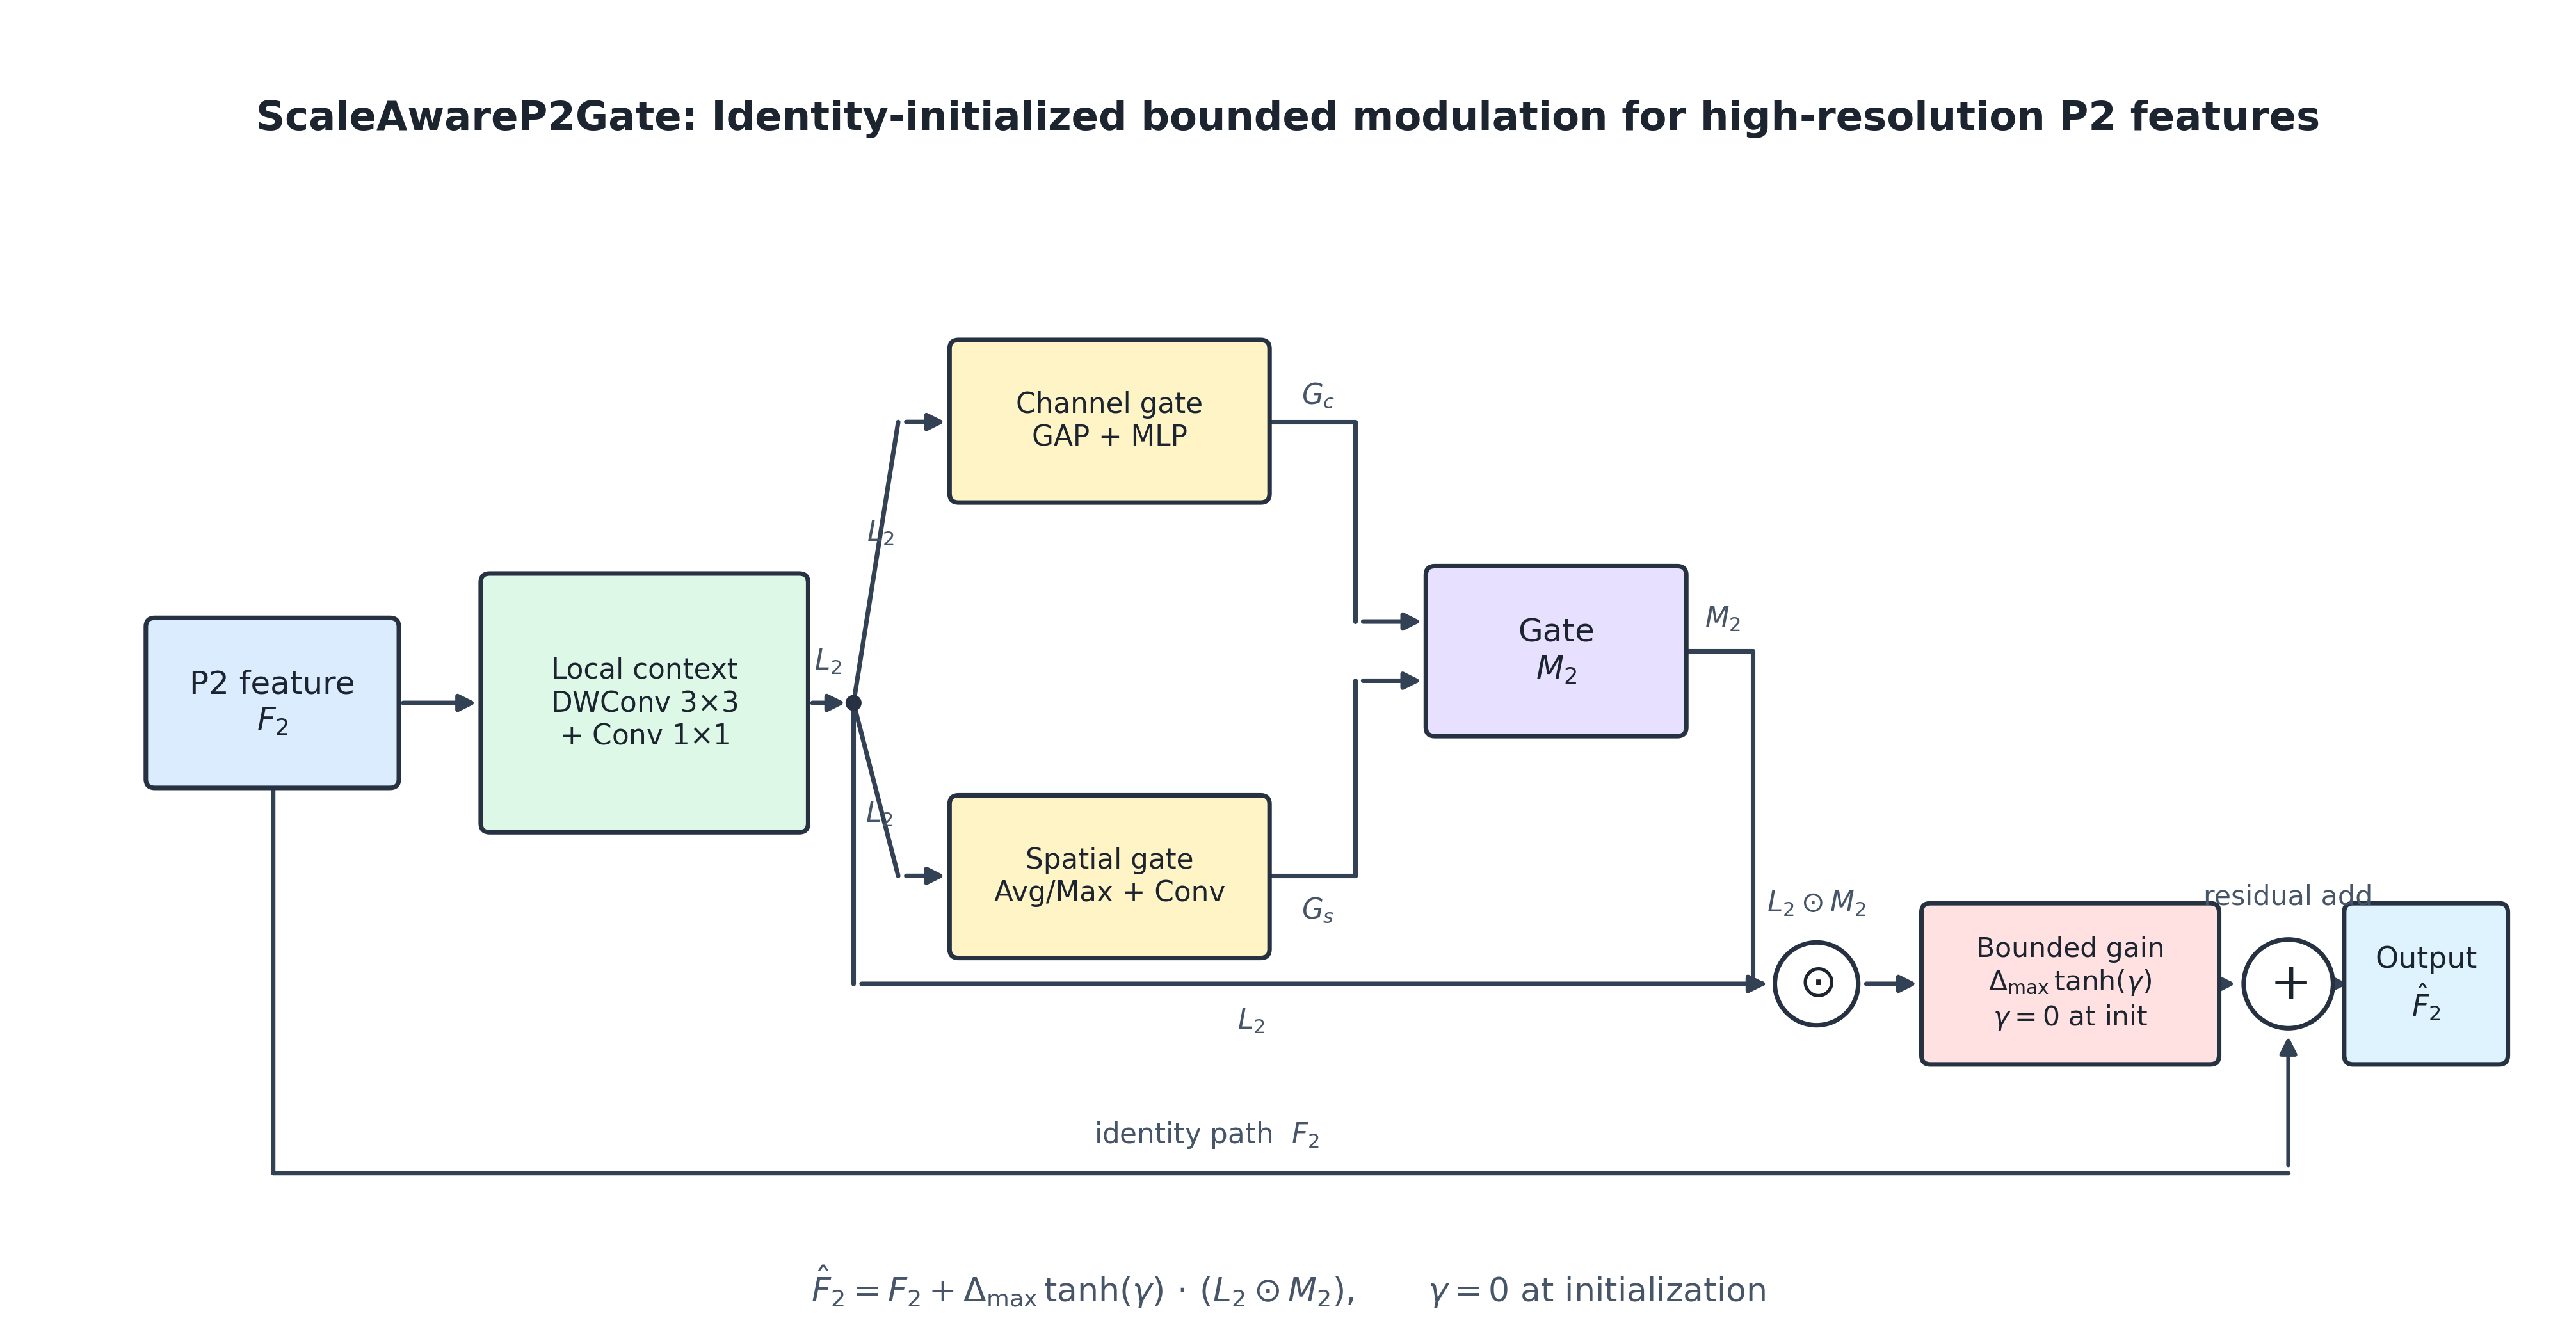
\includegraphics[width=0.96\textwidth]{scalegate_schematic.png}
  \caption{ScaleAwareP2Gate structure. The completed results are used as mixed/negative adaptive-gate evidence rather than as the final method claim.}
  \label{fig:scalegate_schematic}
\end{figure*}

\subsection{Second-Cycle CrossScaleP2P3ConsistencyGate}

The ScaleGate result suggests that self-conditioned P2 modulation is not sufficient: it can preserve a small aggregate gain on VisDrone while reducing small-object diagnostics and failing to improve UAVDT. The second-cycle candidate, CrossScaleP2P3ConsistencyGate (CSGate), therefore conditions shallow P2 detail on neighboring P3 semantic context. Let \(F_2\) be the P2 feature and \(F_3\) be the adjacent P3 feature. After nearest-neighbor alignment, the contextual features are
\begin{equation}
C_2 = g_2(F_2), \qquad C_3 = g_3(\mathrm{Up}(F_3)),
\end{equation}
where \(g_2\) is a local depthwise-separable projection and \(g_3\) is a \(1\times1\) projection. The cross-scale consistency gate is
\begin{equation}
A_{23} = \sigma\left(q([C_2, C_3])\right),
\end{equation}
and the adapted P2 feature is
\begin{equation}
\tilde{F}_2 = F_2 + \lambda A_{23} \odot (C_2 - C_3), \qquad
\lambda = \Delta_{\max}\tanh(\eta).
\end{equation}
Here \(\eta\) is initialized to zero, so the candidate starts from the static P2 path and learns a bounded correction. The module is therefore a controlled hypothesis derived from the ScaleGate failure mode: shallow detail should be modulated with neighboring semantic context rather than with P2-local saliency alone. The completed CSGate evidence is interpreted under this bounded hypothesis: it can be discussed as a cross-scale adaptation candidate because it repairs part of the UAVDT static-P2 degradation and improves VisDrone small-object recall, but it cannot be described as a universally stronger detector.

\subsection{Claim-Bounded Evaluation Protocol}

The framework is intentionally claim-bounded. The implemented variants may support statements about prediction hierarchy, input resolution, feature calibration, and measured efficiency. They do not support cross-dataset robustness, state-of-the-art performance, or universal attention-module improvement unless those statements are supported by complete audited results. This boundary is important because the contribution should be judged not only by the presence of a model change, but by whether the change is consistently supported by fair comparisons and diagnostic metrics.

\section{Experiments and Evidence}

\subsection{Datasets and Metrics}

The completed evidence uses the VisDrone2019-DET validation split. Objects are grouped by area into small, medium, and large bins for diagnostic analysis. The recall/precision table is computed by ground-truth scale groups. The local scale-bin AP table filters ground-truth and predicted boxes by scale bin and should not be described as the official COCO or VisDrone small/medium/large AP protocol. This distinction prevents a local diagnostic from being overstated as an official benchmark metric.

UAVDT is used as the cross-dataset boundary test. It has been downloaded, MD5-checked, reorganized into the project YOLO layout, and verified by the dataset checker. The paper-facing UAVDT rows are exported only from complete 100-epoch runs with local \texttt{results.csv}, \texttt{args.yaml}, and \texttt{weights/best.pt} evidence. Server-side partial metrics are excluded from paper evidence.

\subsection{Implementation Details}

The completed training logs use 100 epochs and seed 42 for the compared VisDrone runs. Nano-scale 960-input runs use batch size 4. The speed protocol uses single-image GPU wall-clock timing with 10 warm-up runs and 100 measured samples. Parameters, GFLOPs, weight size, latency, and FPS are copied from audited CSV files and generated tables. Hardware and software settings are reported from audited experiment records rather than from memory.

\subsection{Reproducibility and Result Integration}

All tables in this manuscript are generated from CSV files under \texttt{paper/tables/}. The LaTeX table sources under \texttt{paper/ieee\_trans/tables/} are generated artifacts and are not edited by hand for numeric changes. UAVDT rows follow the same integration rule: complete runs must reach the configured epoch threshold, be synced to the local workspace, exported into manuscript-safe CSV files, and pass the IEEE table audit before they can be inserted into the result tables. This workflow keeps training progress, exploratory results, and manuscript evidence separate.

\subsection{Main VisDrone Results}

% Auto-generated by tools/export_ieee_tables.py.
% Values are copied from audited CSV files; do not edit numbers by hand.
\begin{table*}[t]
\centering
\caption{Detection results on the VisDrone2019-DET validation set.}
\label{tab:ieee_visdrone_main_results}
\footnotesize
\begin{tabular*}{\textwidth}{@{\extracolsep{\fill}}lrrrrrr@{}}
\hline
Model & Img & Params/M & P & R & mAP50 & mAP50--95 \\
\hline
YOLOv5n & 640 & 2.510 & 0.436 & 0.329 & 0.310 & 0.175 \\
YOLOv8n & 640 & 3.013 & 0.448 & 0.345 & 0.325 & 0.184 \\
YOLOv8n-960 & 960 & 3.013 & 0.536 & 0.419 & 0.420 & 0.251 \\
YOLO11n & 640 & 2.592 & 0.454 & 0.339 & 0.322 & 0.182 \\
YOLO11n-960 & 960 & 2.592 & 0.533 & 0.419 & 0.421 & 0.251 \\
YOLO11n-P2-960 & 960 & 2.894 & 0.538 & 0.421 & 0.424 & 0.256 \\
YOLO11n-P2-CA-960 & 960 & 2.904 & 0.534 & 0.428 & 0.420 & 0.252 \\
YOLO11n-P2-TOFC-960 & 960 & 2.896 & 0.515 & 0.415 & 0.428 & 0.261 \\
YOLO11n-P2-ScaleGate-960 & 960 & 2.896 & 0.519 & 0.414 & 0.429 & 0.261 \\
YOLO11s-960 & 960 & 9.432 & 0.590 & 0.476 & 0.489 & 0.298 \\
\hline
\end{tabular*}
\vspace{1mm}\par\footnotesize All values are traced to \texttt{paper/tables/main\_comparison\_for\_paper.csv}.
\end{table*}


Table~\ref{tab:ieee_visdrone_main_results} shows that increasing the input resolution from 640 to 960 substantially improves YOLO11n. Under the 960-input setting, YOLO11n-P2-960 modestly improves the nano-scale aggregate metrics over YOLO11n-960. YOLO11n-P2-TOFC-960, YOLO11n-P2-ScaleGate-960, and YOLO11n-P2-CSGate-960 have stronger completed nano-scale aggregate metrics than static P2 in the current table, but these findings must be interpreted together with the scale-wise diagnostics below. CSGate reaches 0.272 best mAP50--95 on VisDrone, above static P2 and ScaleGate, while YOLO11s-960 remains the strongest completed reference in absolute accuracy.

\subsection{Efficiency and Complexity}

% Auto-generated by tools/export_ieee_tables.py.
% Values are copied from audited CSV files; do not edit numbers by hand.
\begin{table}[t]
\centering
\caption{Speed and complexity comparison for completed VisDrone models.}
\label{tab:ieee_speed_complexity}
\footnotesize
\begin{tabular}{lrrrrrr}
\hline
Model & Img & Params/M & GFLOPs & MB & Latency/ms & FPS \\
\hline
YOLO11n-960 & 960 & 2.592 & 6.5 & 5.25 & 21.31 & 46.92 \\
YOLO11n-P2-960 & 960 & 2.894 & 10.7 & 6.06 & 22.88 & 43.71 \\
YOLO11n-P2-CA-960 & 960 & 2.904 & 10.7 & 6.09 & 23.36 & 42.82 \\
YOLO11n-P2-TOFC-960 & 960 & 2.896 & 10.8 & 6.07 & 22.61 & 44.23 \\
YOLOv8n-960 & 960 & 3.013 & 8.2 & 5.99 & 20.32 & 49.21 \\
YOLO11s-960 & 960 & 9.432 & 21.6 & 18.32 & 24.02 & 41.63 \\
\hline
\end{tabular}
\vspace{1mm}\par\footnotesize Latency and FPS use the wall-clock protocol recorded in \texttt{paper/tables/speed\_results.csv}.
\end{table}


Table~\ref{tab:ieee_speed_complexity} reports the efficiency side of the comparison. The P2-family variants add parameters and GFLOPs relative to YOLO11n-960. ScaleGate remains close to TOFC and static P2 in model size and local speed under the current protocol, but its accuracy diagnostics do not justify a main-method claim. CSGate further increases the parameter count and GFLOPs because it introduces cross-scale P2/P3 conditioning, so its UAVDT repair must be weighed against the extra computation. The larger YOLO11s-960 model has a much larger parameter count and weight file, which supports a deployment-oriented discussion but not an absolute superiority claim for nano-scale models.

\subsection{Scale-Wise Diagnostics}

% Auto-generated by tools/export_ieee_tables.py.
% Values are copied from audited CSV files; do not edit numbers by hand.
\begin{table*}[t]
\centering
\caption{Scale-wise recall and precision on the VisDrone2019-DET validation set.}
\label{tab:ieee_scale_recall_precision}
\footnotesize
\begin{tabular*}{\textwidth}{@{\extracolsep{\fill}}lrrrrrr@{}}
\hline
Model & S-R & S-P & M-R & M-P & L-R & L-P \\
\hline
YOLO11n-960 & 0.420 & 0.662 & 0.789 & 0.780 & 0.890 & 0.862 \\
YOLO11n-P2-960 & 0.450 & 0.675 & 0.779 & 0.785 & 0.888 & 0.842 \\
YOLO11n-P2-CA-960 & 0.455 & 0.666 & 0.781 & 0.789 & 0.882 & 0.844 \\
YOLOv8n-960 & 0.423 & 0.661 & 0.786 & 0.789 & 0.887 & 0.862 \\
YOLO11s-960 & 0.493 & 0.681 & 0.828 & 0.799 & 0.900 & 0.877 \\
YOLO11n-P2-TOFC-960 & 0.431 & 0.678 & 0.765 & 0.793 & 0.875 & 0.854 \\
YOLO11n-P2-ScaleGate-960 & 0.427 & 0.669 & 0.765 & 0.792 & 0.877 & 0.845 \\
\hline
\end{tabular*}
\vspace{1mm}\par\footnotesize S/M/L denote small, medium, and large GT object groups. This table reports recall/precision, not AP.
\end{table*}


% Auto-generated by tools/export_ieee_tables.py.
% Values are copied from audited CSV files; do not edit numbers by hand.
\begin{table*}[t]
\centering
\caption{Local scale-bin AP on the VisDrone2019-DET validation set.}
\label{tab:ieee_scale_bin_ap}
\footnotesize
\begin{tabular*}{\textwidth}{@{\extracolsep{\fill}}lrrrrrr@{}}
\hline
Model & S-AP50 & S-mAP & M-AP50 & M-mAP & L-AP50 & L-mAP \\
\hline
YOLO11n-960 & 0.230 & 0.116 & 0.453 & 0.310 & 0.578 & 0.459 \\
YOLO11n-P2-960 & 0.248 & 0.132 & 0.438 & 0.301 & 0.456 & 0.369 \\
YOLO11n-P2-CA-960 & 0.239 & 0.126 & 0.438 & 0.301 & 0.419 & 0.348 \\
YOLOv8n-960 & 0.238 & 0.122 & 0.459 & 0.313 & 0.528 & 0.440 \\
YOLO11s-960 & 0.303 & 0.159 & 0.524 & 0.367 & 0.562 & 0.473 \\
YOLO11n-P2-TOFC-960 & 0.230 & 0.121 & 0.425 & 0.288 & 0.422 & 0.334 \\
YOLO11n-P2-ScaleGate-960 & 0.225 & 0.119 & 0.427 & 0.288 & 0.446 & 0.357 \\
\hline
\end{tabular*}
\vspace{1mm}\par\footnotesize S/M/L denote small, medium, and large object groups. This diagnostic uses local scale-bin filtering and is not an official COCO or VisDrone small-object AP metric.
\end{table*}


Tables~\ref{tab:ieee_scale_recall_precision} and~\ref{tab:ieee_scale_bin_ap} are the central evidence for the small-object motivation. YOLO11n-P2-960 improves small-object recall and local small-bin AP over YOLO11n-960, while the gains are not uniform across all object sizes. CoordAttention changes the recall and precision behavior, and TOFC improves aggregate mAP but not the strongest small-bin diagnostic relative to P2-only. ScaleGate further illustrates the risk of relying on aggregate mAP alone: despite its VisDrone aggregate gain, its small recall is 0.427 and local small-bin AP50 is 0.225, both below static P2. CSGate changes this pattern: it raises small-object recall to 0.456, above static P2, but its local small-bin AP50 is 0.243, slightly below static P2 and above ScaleGate. Fig.~\ref{fig:scale_recall_visdrone} visualizes the recall trend across object scales.

\begin{figure}[t]
  \centering
  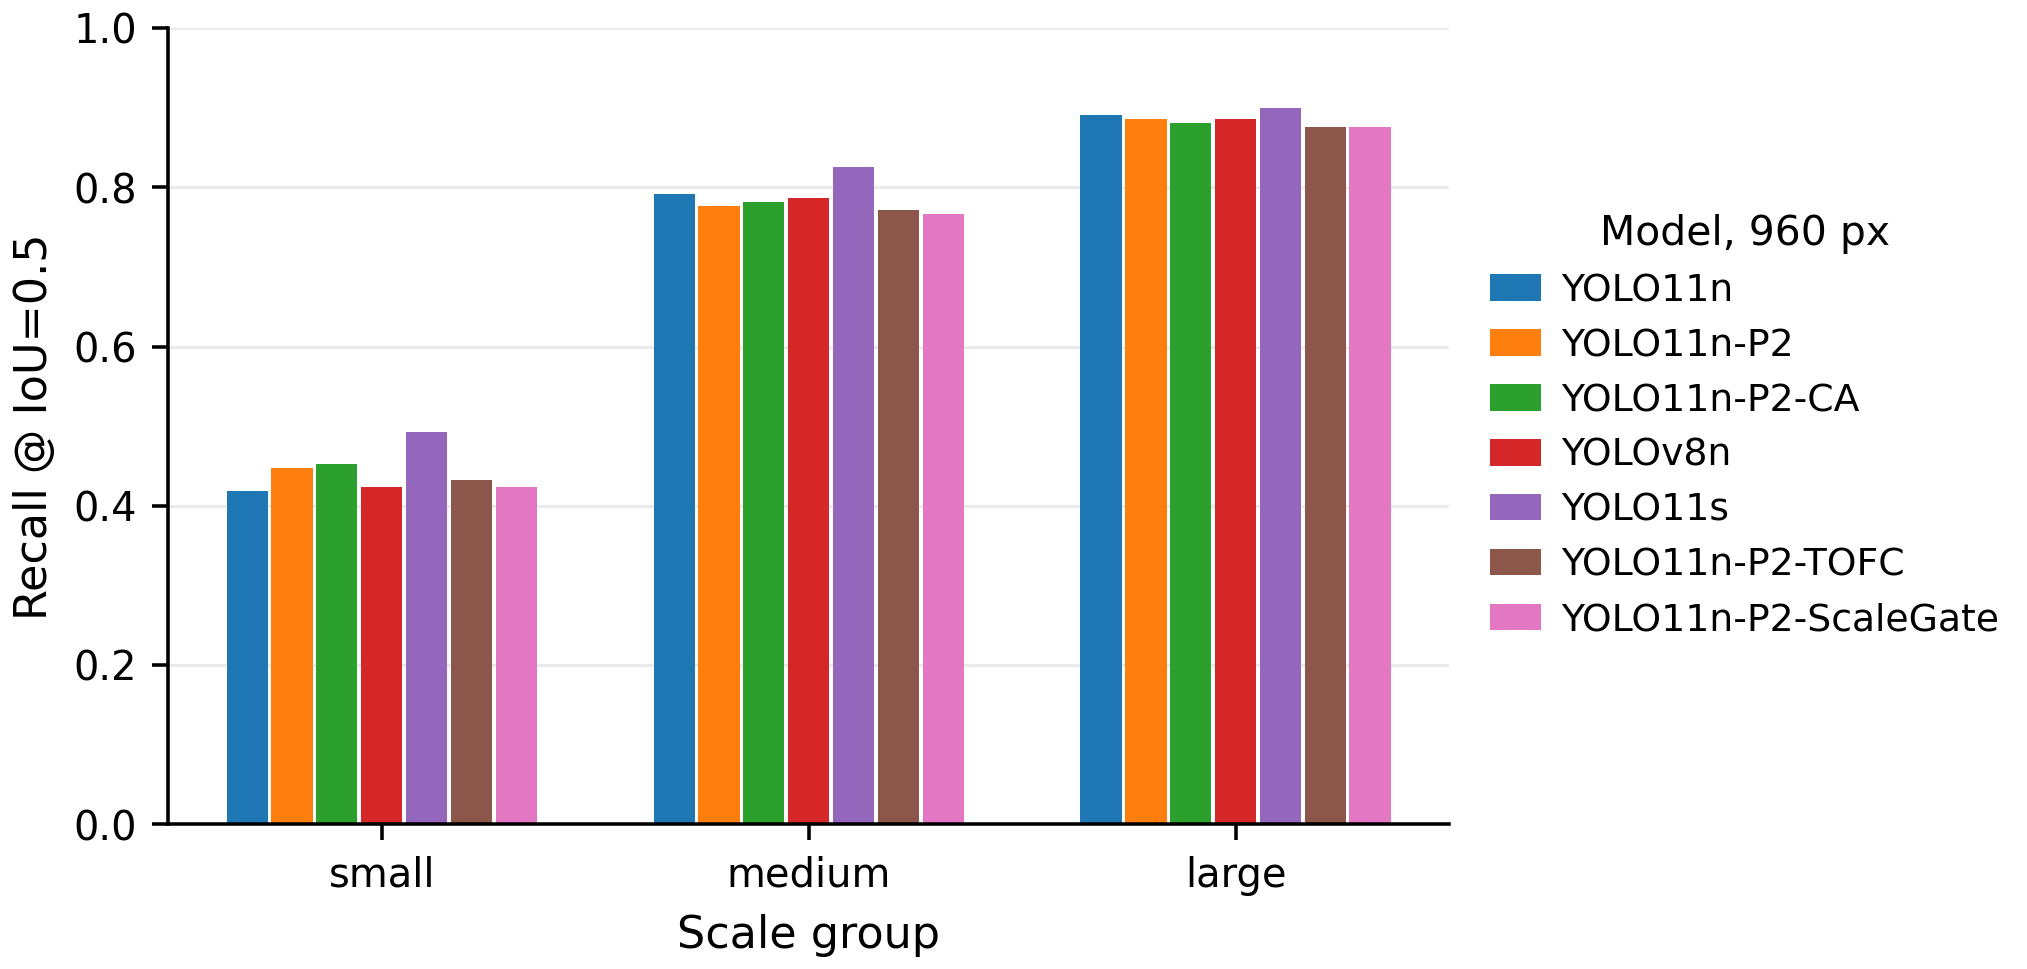
\includegraphics[width=\linewidth]{ieee_scale_recall_visdrone.png}
  \caption{Scale-wise recall on the VisDrone2019-DET validation set. The figure is generated from audited scale-group CSV files.}
  \label{fig:scale_recall_visdrone}
\end{figure}

\subsection{Cross-Dataset Boundary Gate}

% Auto-generated by tools/export_ieee_uavdt_results.py.
% Values are copied from complete local UAVDT runs only.
\begin{table*}[t]
\centering
\caption{Detection results on the UAVDT validation set.}
\label{tab:ieee_uavdt_results}
\footnotesize
\begin{tabular*}{0.82\textwidth}{@{\extracolsep{\fill}}lrrrrr}
\hline
Model & Img & P & R & mAP50 & mAP50--95 \\
\hline
YOLO11n-960 & 960 & 0.85840 & 0.84102 & 0.88444 & 0.59081 \\
YOLO11n-P2-960 & 960 & 0.80931 & 0.81385 & 0.83711 & 0.53905 \\
YOLOv8n-960 & 960 & 0.88214 & 0.84659 & 0.88983 & 0.59487 \\
YOLO11s-960 & 960 & 0.87458 & 0.87049 & 0.89756 & 0.60819 \\
YOLO11n-P2-ScaleGate-960 & 960 & 0.77939 & 0.82089 & 0.83056 & 0.53758 \\
\hline
\end{tabular*}
\vspace{1mm}\par\footnotesize Values are exported only from runs with complete training evidence.
\end{table*}


UAVDT is used as the cross-dataset validation dataset for the boundary analysis. Table~\ref{tab:ieee_uavdt_results} reports the required comparison set: YOLO11n-960, YOLO11n-P2-960, YOLOv8n-960, YOLO11s-960, ScaleGate, and CSGate. Unlike the VisDrone result, YOLO11n-P2-960 is weaker than the resolution-matched YOLO11n-960 baseline on UAVDT, decreasing mAP50--95 from 0.591 to 0.539 and mAP50 from 0.884 to 0.837. YOLOv8n-960 and YOLO11s-960 also exceed the P2 variant, with mAP50--95 values of 0.595 and 0.608, respectively. ScaleGate obtains 0.538 mAP50--95 and 0.831 mAP50, so it does not repair the static-P2 boundary. CSGate raises UAVDT mAP50--95 to 0.567 and mAP50 to 0.865, recovering 54.8\% of the mAP50--95 gap between static P2 and YOLO11n-960. It therefore provides evidence that cross-scale P2/P3 conditioning is more appropriate than P2-local gating for this boundary case. However, CSGate remains below YOLO11n-960, YOLOv8n-960, and YOLO11s-960 on UAVDT, so the result supports partial repair rather than cross-dataset superiority.

\section{Discussion: Benefits, Costs, and Boundaries}

The completed VisDrone results suggest that high-resolution input and a P2 prediction branch can improve small-object diagnostics for a compact YOLO11n detector. This is consistent with the intuition that shallow features preserve spatial detail that can be lost in deeper low-resolution maps. However, the aggregate gains are modest and the scale-wise results show trade-offs across object sizes. The UAVDT results further show that the VisDrone P2 gain is not a transferable guarantee: under the current UAVDT setting, YOLO11n-P2-960 is weaker than YOLO11n-960, YOLOv8n-960, and YOLO11s-960. The key finding is therefore not that P2 is universally better, but that high-resolution prediction can shift detector behavior toward small-object sensitivity in some data regimes while also creating cost and generalization risks.

The comparison with YOLO11s-960 is important. A larger model remains stronger in absolute accuracy on both VisDrone and UAVDT, so the paper should not be framed as a nano detector outperforming larger detectors. Instead, YOLO11s acts as a capacity boundary. It shows what is gained by staying near the nano regime and what is lost relative to a larger model. The UAVDT table also shows that YOLOv8n-960 is a strong lightweight reference on this dataset, which prevents the analysis from becoming an internal YOLO11-only comparison.

The completed attention and calibration results also require careful wording. CoordAttention changes the precision-recall balance but does not dominate all aggregate metrics. TOFC currently improves aggregate nano-scale mAP on VisDrone, but its small-object diagnostic metrics do not exceed the P2-only model and it has not been validated on UAVDT in the current comparison set. CSGate improves VisDrone aggregate mAP over static P2 and ScaleGate and repairs part of the UAVDT degradation, but it also increases computation and does not dominate local small-bin AP. Therefore, the method choice cannot be made from a single aggregate score alone; it must be made from the combined evidence of aggregate accuracy, small-object diagnostics, complexity, and cross-dataset behavior. The local scale-bin diagnostics are included for this reason: they reveal whether an apparent aggregate gain actually corresponds to the small-object motivation.

The audited UAVDT results resolve the scope of the current P2 finding. Because the P2 trend is inconsistent across VisDrone and UAVDT, the safest conclusion is dataset-dependent behavior rather than cross-dataset robustness. This does not make the VisDrone scale-wise analysis useless; it clarifies the condition under which the mechanism is helpful and identifies when a simpler or larger baseline is preferable. Under this framing, UAVDT strengthens the validity-boundary analysis rather than the method-superiority claim.

The completed ScaleGate experiment is an informative negative result. ScaleGate raises the VisDrone aggregate score slightly but weakens the small-object diagnostics that motivated the method and remains below the key UAVDT baselines. This failure mode points to a more specific hypothesis: shallow P2 detail should not be gated only by its own local saliency, but should be checked against neighboring semantic context. The completed CSGate evidence supports this hypothesis in a bounded way. It passes the predeclared cross-dataset repair route by improving UAVDT mAP50--95 from 0.539 to 0.567 and preserving VisDrone aggregate accuracy, and it passes the small-object diagnostic route by improving VisDrone small recall from 0.450 to 0.456. It fails the stricter balanced-gain route because local small-bin AP50 is 0.243, slightly below the static-P2 value of 0.248. Thus the final method claim should emphasize cross-scale adaptation as a partial repair mechanism, not a universally dominant detector.

\section{Conclusion}

This work studies high-resolution prediction for lightweight UAV small-object detection. The completed VisDrone2019-DET evidence shows that increasing input resolution is the largest source of improvement for YOLO11n, and that adding a P2 branch under matched 960 input further improves several small-object diagnostics. The same evidence also shows important boundaries: P2 increases computation, benefits are not uniform across all object scales, CoordAttention and TOFC have metric-dependent effects, and YOLO11s remains stronger in absolute accuracy. UAVDT further narrows the conclusion: YOLO11n-P2-960 does not outperform YOLO11n-960, YOLOv8n-960, or YOLO11s-960 on the cross-dataset validation setting. ScaleAwareP2Gate also fails the predeclared main-method decision gate, because it does not preserve the key small-object diagnostics or repair UAVDT. CrossScaleP2P3ConsistencyGate improves VisDrone aggregate accuracy, raises small-object recall, and repairs part of the UAVDT static-P2 degradation, but it remains below the strongest UAVDT baselines and slightly below static P2 in local small-bin AP50. The final conclusion is therefore a bounded method claim: cross-scale P2/P3 adaptation is a useful partial repair mechanism for lightweight high-resolution prediction, while the broader problem still requires stronger evidence before a cross-dataset superiority claim can be made.

\bibliographystyle{IEEEtran}
\bibliography{references_seed}

\end{document}
